\chapter{Methodological Safety Discrimination Beyond Evaluations}
\label{chap:probes}
 Although we focus primarily on safety evaluations in this thesis, methodological safety discrimination does not apply exclusively to those. Methods for training and monitoring safeguards may equally be affected. In this chapter, we present a small experiment building on case study \ref{cs:social_syc} about social sycophancy across languages, in which we investigated differences in the performance and transferability of linear probes across languages. Through this we hope to draw attention to the need to further study whether and how methods developed for making models safer may not protect all users equally.

 
\section{Case Study: Cross-lingual Generalisation of Linear Probes for Social Sycophancy Detection}

Linear probes – small linear classifiers trained on residual stream activations of models – have proven to be surprisingly simple and useful for monitoring LLMs' output for various behaviours and concepts. In contrast to LLM-based monitors checking the chain-of-thought and response of the target model at hand, activation-based monitoring is often cheaper and has lower latency at similar performance levels~\cite{mckenzie2025detecting-612}. However, the question of cross-lingual transfer and performance of these monitors is particularly pertinent. Although evidence suggests LLMs develop language-independent concept representations in their middle layers \cite{muller-etal-2021-first, wang2025lost-9a1, liu-niehues-2025-middle}, this shared space may remain structurally anchored to English \cite{wendler2024do-f67}, and probes trained on English data suffer accuracy degradation in other languages \cite{li2024exploring-99e}. For the case of social sycophancy, we will in the following aim to answer to what extent linear probes for detecting social sycophancy trained in one language are effective in detection in other languages. 

\subsection{Methods}
In this experiment, we restricted our representational analysis  to \textit{representation reading} – \textit{reading} from the residual stream activations whether the model is responding sycophantically or honestly. For this, we explored and compared two types of linear probes: a \textit{difference-in-means}-based probe \cite{belrose2023diff-in-means-196} (subsequently MM-probe) and a logistic regression probe (LR-probe). 

Building on the dataset from Section \ref{sec:syc_data}, we extended our multilingual ELEPHANT version by 300 prompts per language for a training dataset following the same translation approach as described before. 
We then trained both types of probes using contrastive pairs of prompts from this training dataset (n\_pairs = 300/language) with forced token responses (signalling either sycophancy or honesty, see Appendix \ref{app:verdicts}). We collected activations from the residual stream of Qwen3-14B across layers 5 to 35 following prior work \cite{panickssery2023steering-417} and averaged activations across the full response sequence after finding that single token positions performed poorly. 

Apart from training probes on activations of monolingual datasets, we also trained and tested "mixed" probes, based on activations from multilingual datasets containing all eight languages in equal parts.

For the MM-probe, we computed a difference-in-means direction $\mathbf{d}$:
\begin{align*}
\mathbf{d} = \frac{1}{n_{\text{honest}}}\sum_{y_i=1 }\mathbf{x}_i - \frac{1}{n_{\text{sycophantic}}}\sum_{y_i=0}\mathbf{x}_i
\end{align*}
With this we can classify any activation vector $\mathbf{x}$ by passing its dot product with $\mathbf{d}$ through the logistic sigmoid function and using an appropriate probability threshold ($p(y = \text{honest}) = \sigma(\mathbf{x} \cdot \mathbf{d})$).

For the LR-probe, we trained a regular logistic regression classifier with $L_2$-regularization ($C=0.1$) on the feature-wise standardised contrastive activation pairs. 

We trained probes on each layer's average activations and evaluated performance using ROC-AUC-Score on activations from the on-policy responses collected in the test set from Section \ref{sec:syc_data}. We chose ROC-AUC as performance measure to handle the class imbalance  \cite{angelotti2024closer-262} in our test set. 

\subsection{Results}

\begin{figure*}[h]
  \centering
  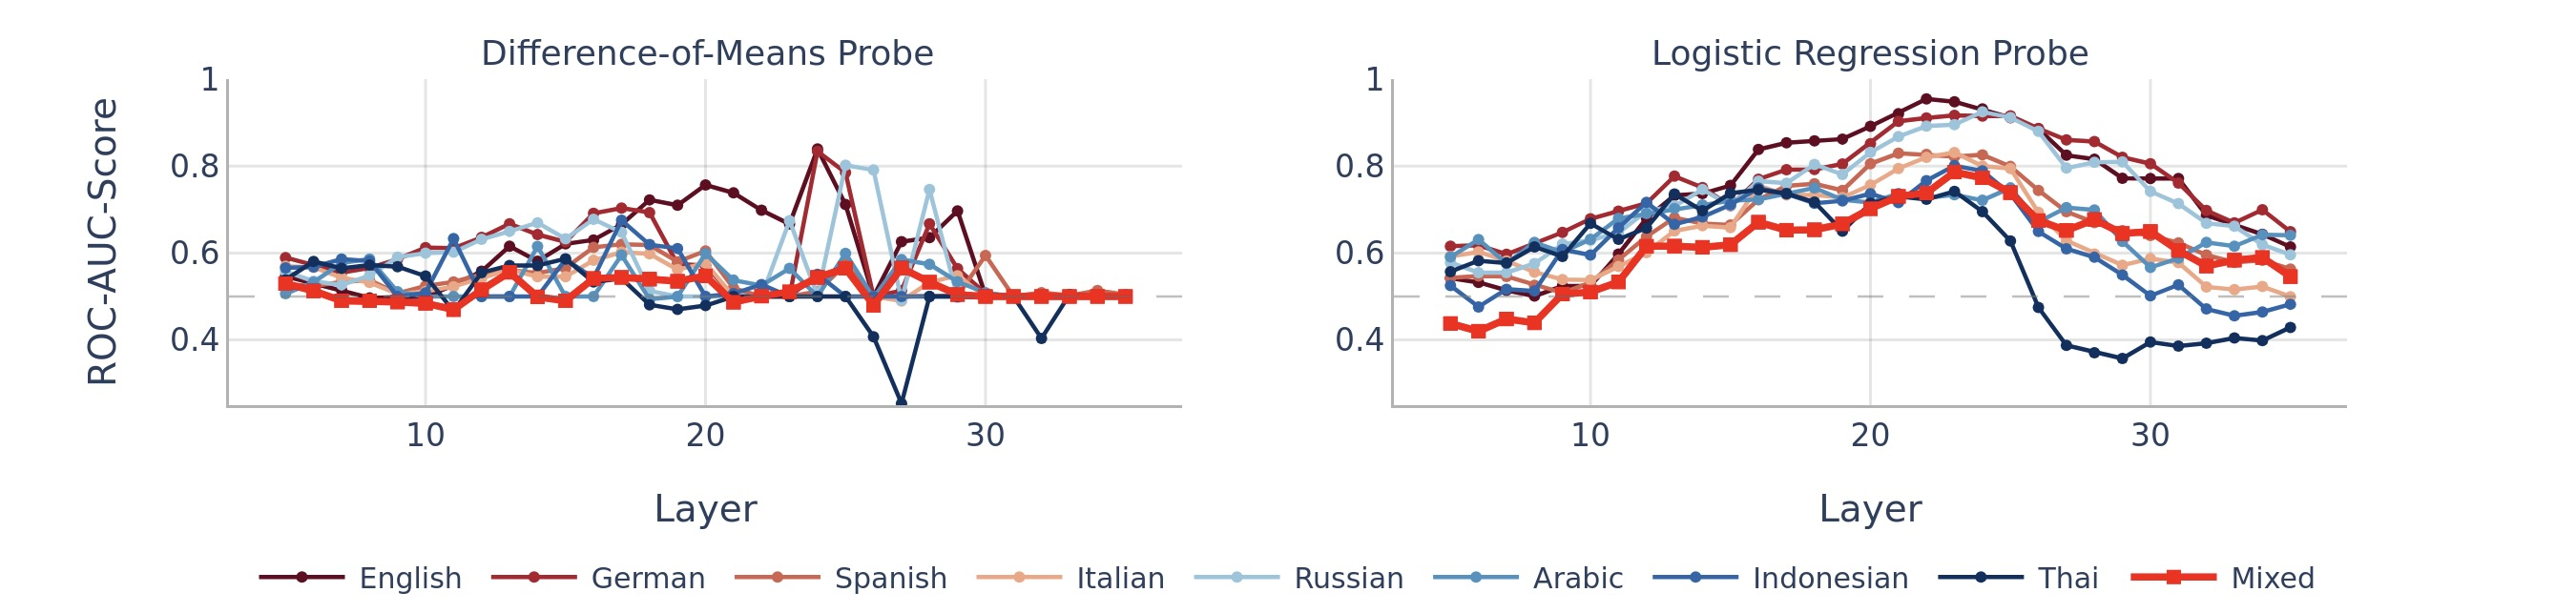
\includegraphics[width=\textwidth]{figures/rq2_layers.jpeg}
  \caption{Layer-wise comparison of probe performances (measured by ROC-AUC) for different languages. Evaluation happened in the same language as training.}
    \label{fig:rq2_layers}
\end{figure*}

\begin{figure*}[h]
  \centering
  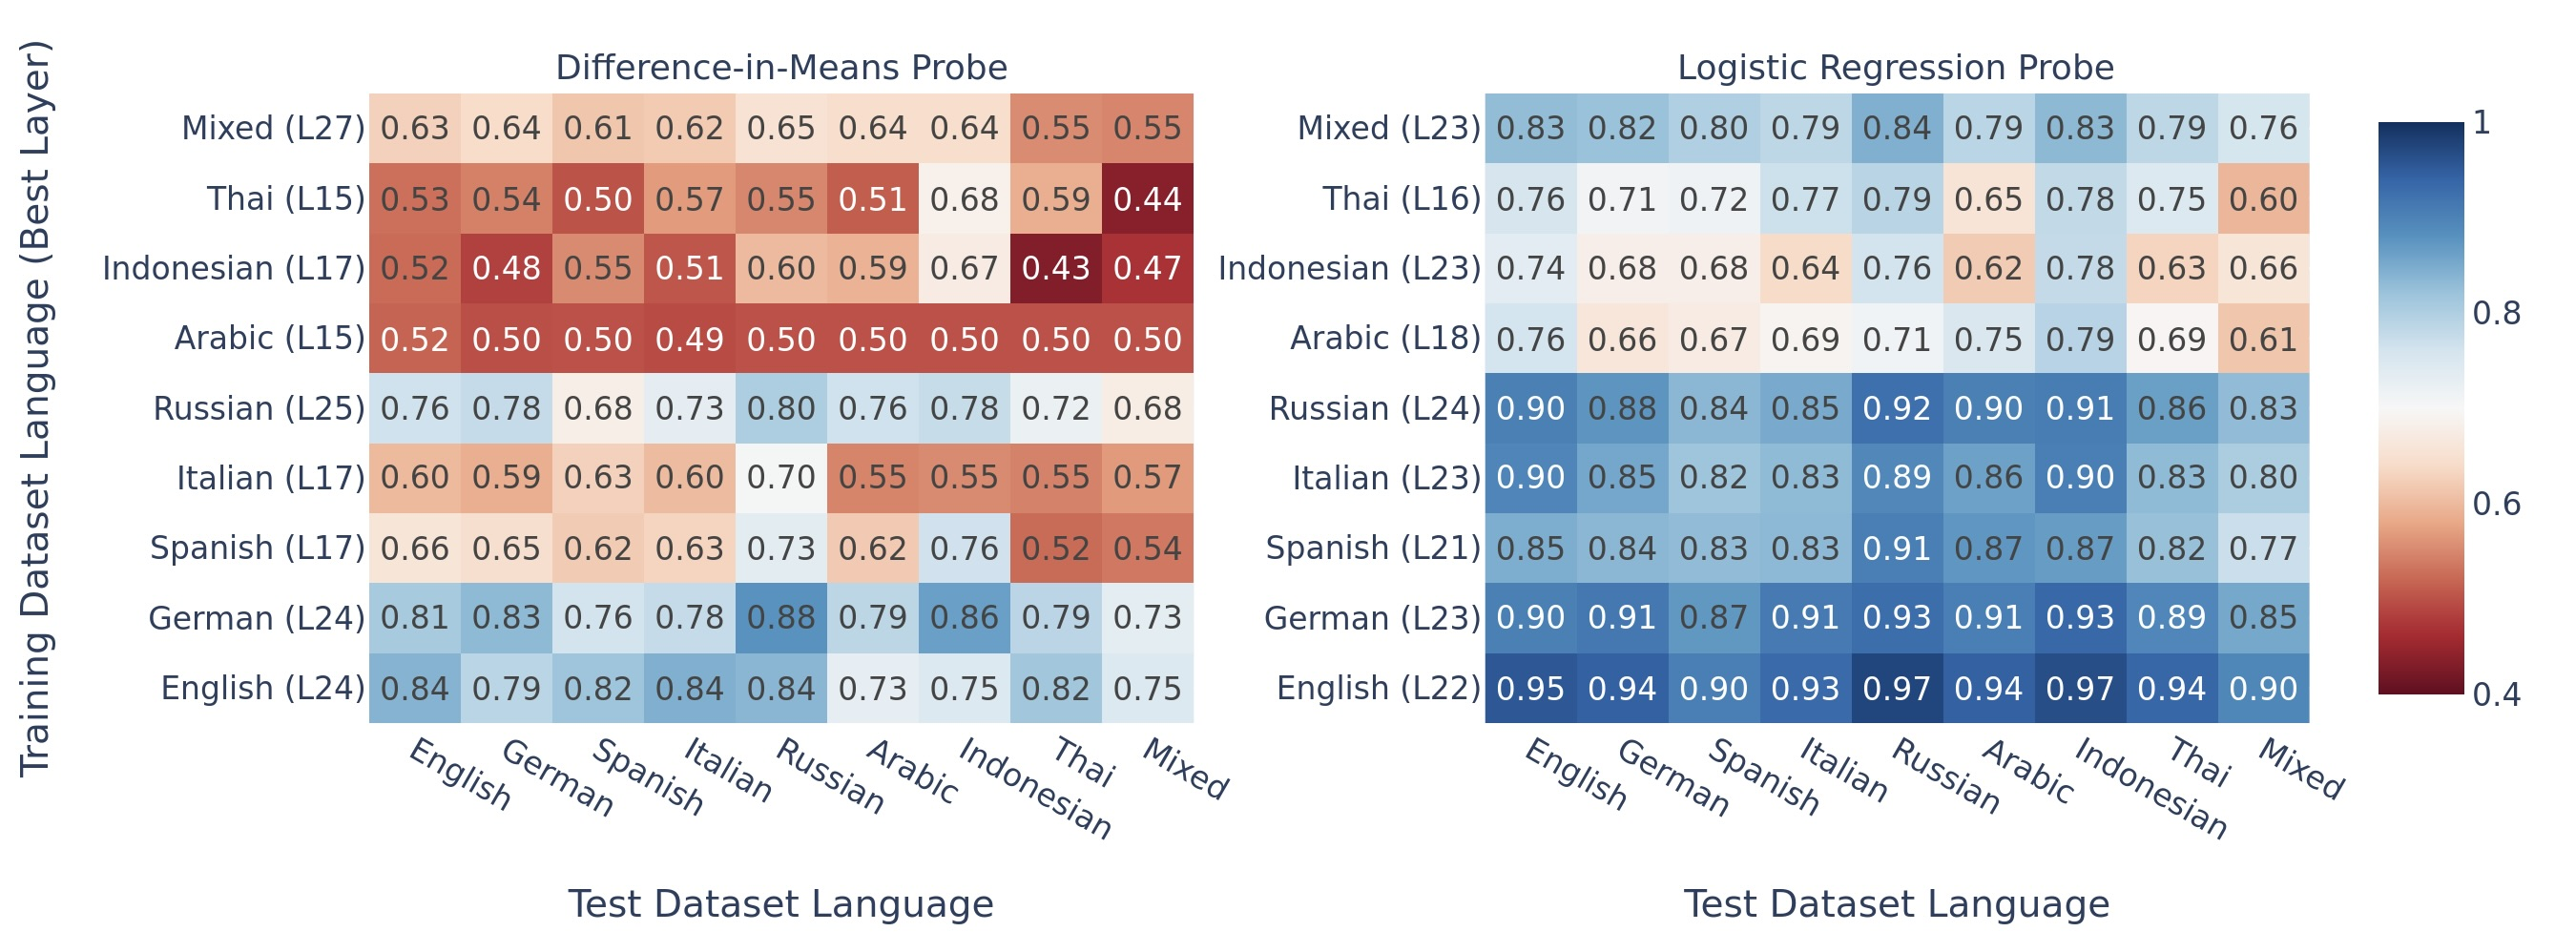
\includegraphics[width=\textwidth]{figures/rq2_best_layer.jpeg}
  \caption{Cross-lingual probe generalisation of the best performing probe per language. All probes show peak performance around the middle layers of the model (layers 15--27 of 40) and LR-probes generally outperform MM-probes.}
    \label{fig:best_layer}
\end{figure*}
\begin{figure*}[h]
  \centering
  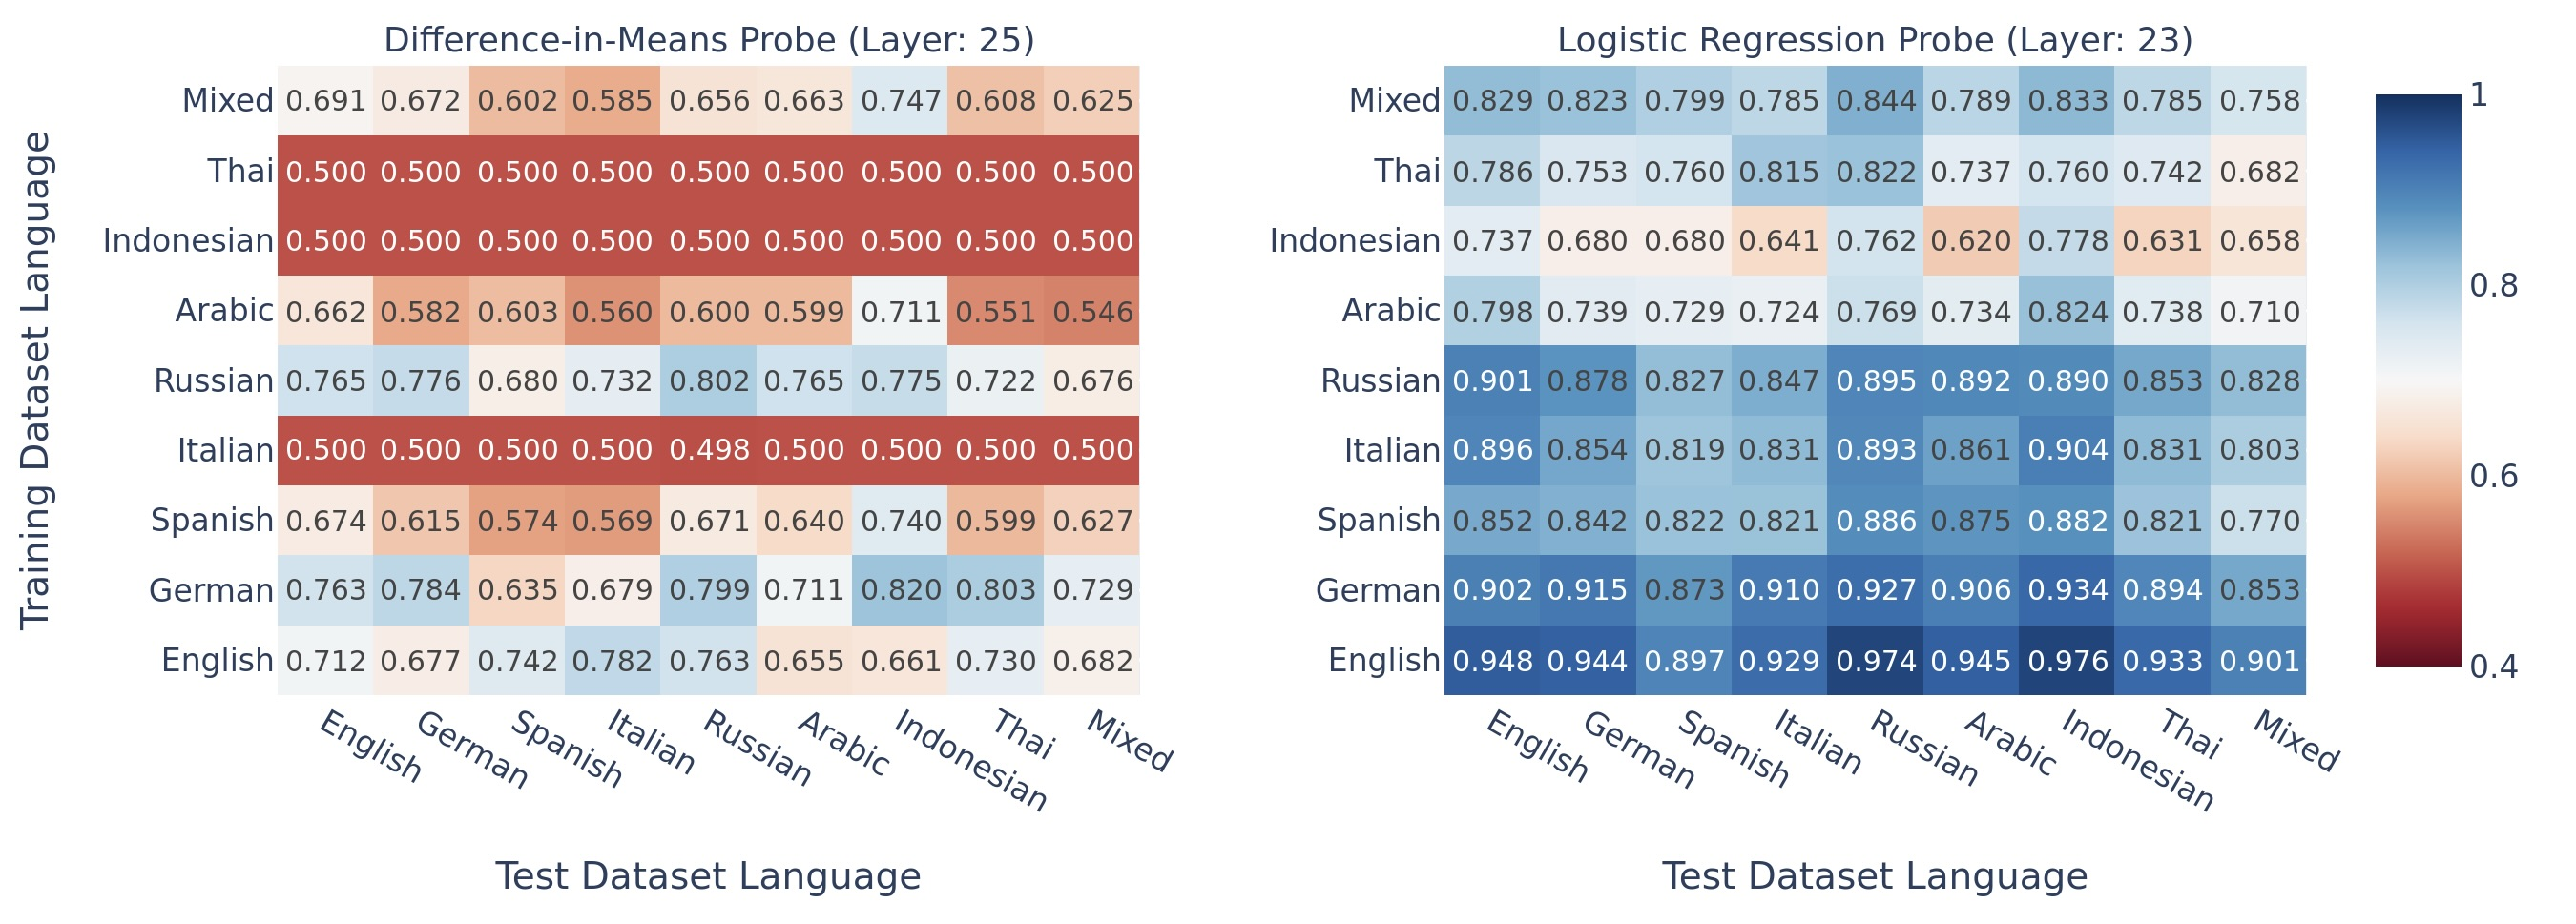
\includegraphics[width=\textwidth]{figures/rq2_universal_layer.jpeg}
  \caption{Cross-lingual probe generalisation of the universally best layer across languages. High-resource languages show generally better performance and transferability than mid-resource languages and LR-probes generally outperform MM-probes.}
    \label{fig:universal_layer}
\end{figure*}

\subsubsection{Within-language performance}
LR-probes largely outperformed MM-probes, both in peak performance and in consistency across layers (Figure~\ref{fig:rq2_layers}). When training and testing in the same language, English probes performed best, followed by the linguistically close languages German, Spanish, and Italian. Russian performed comparably to German, whereas Arabic, Indonesian, and Thai showed markedly lower performance. This ranking correlated strongly with each language's share of available internet text \cite{wikipedianoyearlanguages-eb1} and hence likely its representation in Qwen3-14B's training data.

\subsubsection{Cross-lingual generalisation}
These resource-level patterns persisted when evaluating probes across languages (Figure~\ref{fig:best_layer} and \ref{fig:universal_layer}). English and German probes, both from high-resource Germanic languages, generalised best to all other languages, followed by Russian and the Romance-language probes (Spanish and Italian). Probes from the three mid-resource languages, Arabic, Indonesian, and Thai ($<1\%$ of internet text, as classified in Chapter \ref{chap:translations}), generalised as poorly to other languages as they performed within their own. We found similar patterns when holding the layer constant rather than selecting the best layer per language (see Appendix~\ref{app:universal_layer}). However, we cannot fully rule out that translation artifacts contribute to this degradation.

\subsubsection{Probe direction similarity.}
Probe directions from linguistically close languages exhibited high cosine similarity (${\sim}0.8$), while those from more distant languages were lower (${\sim}0.5$; full pairwise similarity matrices in Appendix~\ref{app:universal_layer}, Tables~\ref{tab:mm_cosim} and \ref{tab:lr_cosim}). Notably, English and Russian directions had a similarity of only $0.65$ despite both generalising well. This suggests that strong generalisation does not require similar probe directions or that different social sycophancy directions exist within the model.

\subsubsection{Mixed-language probe.}
The \textit{mixed}-probe performed between the high- and mid-resource languages, likely because mixing mid-resource activations introduces noise into the otherwise cleaner high-resource signal.


\subsection{Activation-based Monitoring}
In this chapter, we experimented with using linear activation probes to monitor for sycophancy in LLMs' responses as an alternative to the LLM-based monitoring and judging discussed in the previous chapters. However, linear activation probes also need to be trained on certain data, which, as we have seen through our experiments, may influence the quality and generalisability of the probe much more than we expected. This might come as no surprise from the point of view of a traditional ML scientist, but seems less salient to the field of representation engineering, given the lack of prior literature conducting similar experiments to ours in this chapter.
Given that we only used one rather small model, a limited set of languages, and our naive translation approach from Chapter \ref{chap:translations}, we are cautious about generalising our results, but indeed they might point to an understudied problem calling for broader experiments and attention. Activation-based monitoring is used in production safeguarding and evaluations at AI labs. Although English-trained probes transfer best, and English is likely the default training data language, our results show that this should not be taken for granted, and we recommend validating probe quality on multilingual data to avoid methodological safety discrimination in safeguard tooling. As with the previous chapters, this chapter uncovered potential gaps in demographic coverage rather than fixing them. In the following chapter, we will discuss all our findings and their limitations together, as well as what future work should address.




